\documentclass{article}
\usepackage{tikz}
\begin{document}
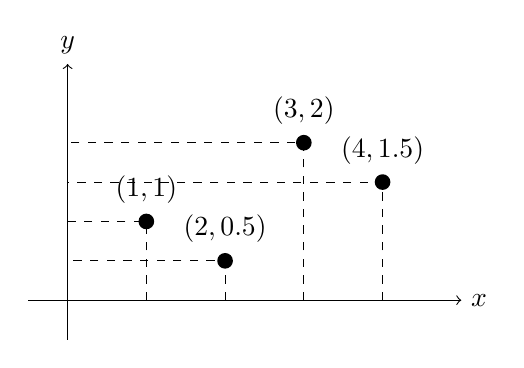
\begin{tikzpicture}
  % Axes
  \draw[->] (-0.5,0) -- (5,0) node[right] {$x$};
  \draw[->] (0,-0.5) -- (0,3) node[above] {$y$};

  % Data points
  \draw (1,1) node[circle,fill,inner sep=2pt,label=above:{$(1,1)$}] {};
  \draw (2,0.5) node[circle,fill,inner sep=2pt,label=above:{$(2,0.5)$}] {};
  \draw (3,2) node[circle,fill,inner sep=2pt,label=above:{$(3,2)$}] {};
  \draw (4,1.5) node[circle,fill,inner sep=2pt,label=above:{$(4,1.5)$}] {};

  % Grid lines
  \draw[dashed] (1,0) -- (1,1) -- (0,1);
  \draw[dashed] (2,0) -- (2,0.5) -- (0,0.5);
  \draw[dashed] (3,0) -- (3,2) -- (0,2);
  \draw[dashed] (4,0) -- (4,1.5) -- (0,1.5);
\end{tikzpicture}
\end{document}
